% arguelles v2.3.0
% author: Michele Piazzai
% contact: michele.piazzai@uc3m.es
% license: MIT

% Copied from GitHub: https://github.com/piazzai/arguelles


\documentclass[compress,12pt]{beamer}
\hypersetup{ 
     colorlinks=true,
     linkcolor=white,
     filecolor=white,
     citecolor = black,
     urlcolor=blue,
     } 

\usetheme{Arguelles}

\tcbset{
    newspaper/.style={
        colback=white, % cor de fundo
        colframe=lightgray, % cor da borda
        fonttitle=\bfseries, % fonte do título
        coltitle=darkblue, % cor do título
        colbacktitle=lightblue, % cor de fundo do título
        toptitle=3pt, % espaço entre o topo do bloco e o título
        bottomtitle=1pt, % espaço entre o título e o conteúdo
        left=5pt, % margem esquerda
        right=5pt, % margem direita
        top=5pt, % margem superior
        bottom=5pt, % margem inferior
        boxsep=0pt, % espaçamento interno
        arc=0pt % estilo das bordas (0pt para retangular)
    }
}

\usepackage{tikz}
\usetikzlibrary{shadows.blur}

% Definição de cores
\definecolor{lightblue}{RGB}{54,69,79}
\definecolor{charcoal}{RGB}{33, 37, 41}
\definecolor{darkblue}{RGB}{0,51,102}

% Estilo para o bloco
\setbeamercolor{block title}{bg=charcoal,fg=white}
\setbeamercolor{block body}{bg=lightblue,fg=white}

\setbeamertemplate{blocks}[rounded][shadow=true]


\title{Dados Tendenciosos e Desonestidade Informativa}
\subtitle{}
\event{Trabalho 01 - Introdução à Ciência de Dados}
\author{Henrique Beltrão, Carlos Daniel, Davi Nunes, Luís Filipe}
% \institute{Fundação Getúlio Vargas - EMAp}
\institute{
\includegraphics[scale=0.4]{Imagens/EMAP.png}}

\begin{document}

\frame[plain]{\titlepage}

% INICIO HENRIQUE

\Section{Henrique}

\begin{frame}
    \frametitle{Twitter, Dados Reais, e a Direita Alternativa}
    \framesubtitle{Henrique Beltrão}
    \textit{Impactos da nova política de "Liberdade de Expressão" no Twitter (X):}
    \begin{itemize}
        \item Ascenção de grupos e páginas da extrema-direita americana;
        \item Desconexão com a realidade;
        \item "Nós contra eles" e "Reais vítimas";
        \item Disseminação do ódio na rede.
    \end{itemize}
\end{frame}

\begin{frame}
    \frametitle{Radicalização Política nas Redes Sociais}
    \centering
        \begin{columns}
        
        \column{0.5\textwidth}
            \centering
            
            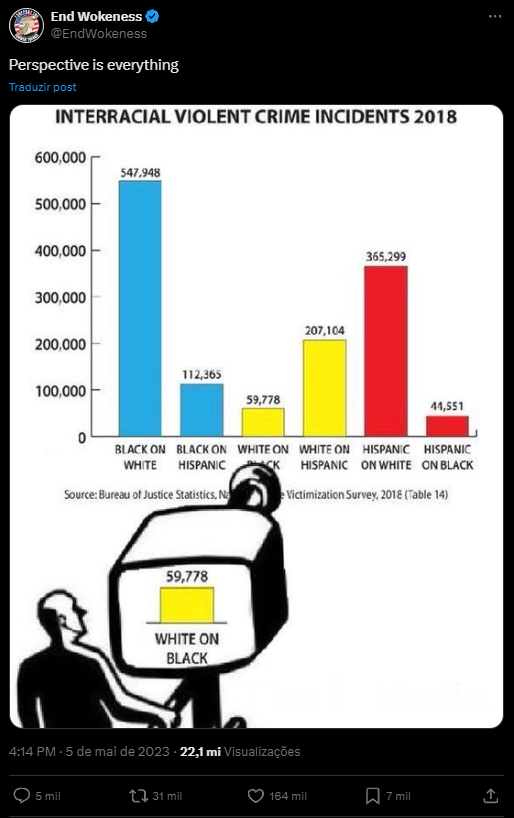
\includegraphics[width=49mm]{Imagens/EndWokeness.png}
            
        \column{0.5\textwidth}
            \centering
            
            \begin{block}{}
                \textit{"Perspectiva é tudo"} \\
                Objetivo do autor:
                \begin{itemize}
                    \item "Pessoas brancas são as reais oprimidas da sociedade";
                    \item "A mídia esconde essa 'verdade factual'";
                    \item "Pessoas diferentes são perigosas";
                    \item Radicalizar a juventude suburbana.
                \end{itemize}
            \end{block}
            Fonte: \href{https://x.com/EndWokeness/status/1654565227701125122?s=20}{\textit{Postagem no X}}
            
        \end{columns}
\end{frame}

\begin{frame}
    \frametitle{OS DADOS}
    De fato, são verdadeiros. Contudo:
    \begin{itemize}
        \item Não representam maioria de crimes violentos (que ocorrem entre indivíduos da mesma raça $\rightarrow \textrm{espaço físico)}$;
    \end{itemize}
    \centering
    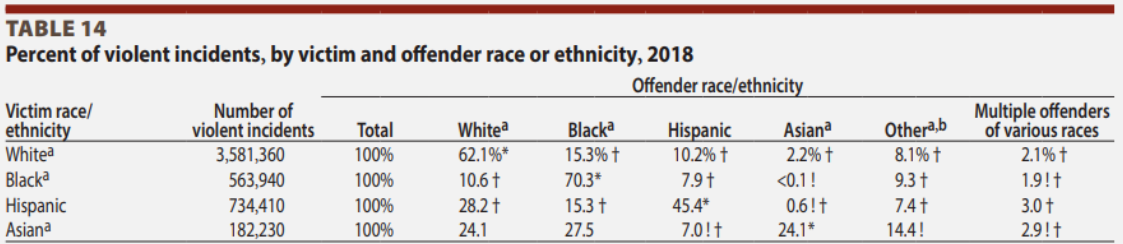
\includegraphics[width=108mm]{Imagens/Table 14 (2018).png}

    Fonte: \href{https://bjs.ojp.gov/content/pub/pdf/cv18.pdf}{\textit{Bureau of Justice Statistics, 2018 (Criminal Victimization)}}
\end{frame}

\begin{frame}
    \frametitle{OS DADOS}
    \centering
    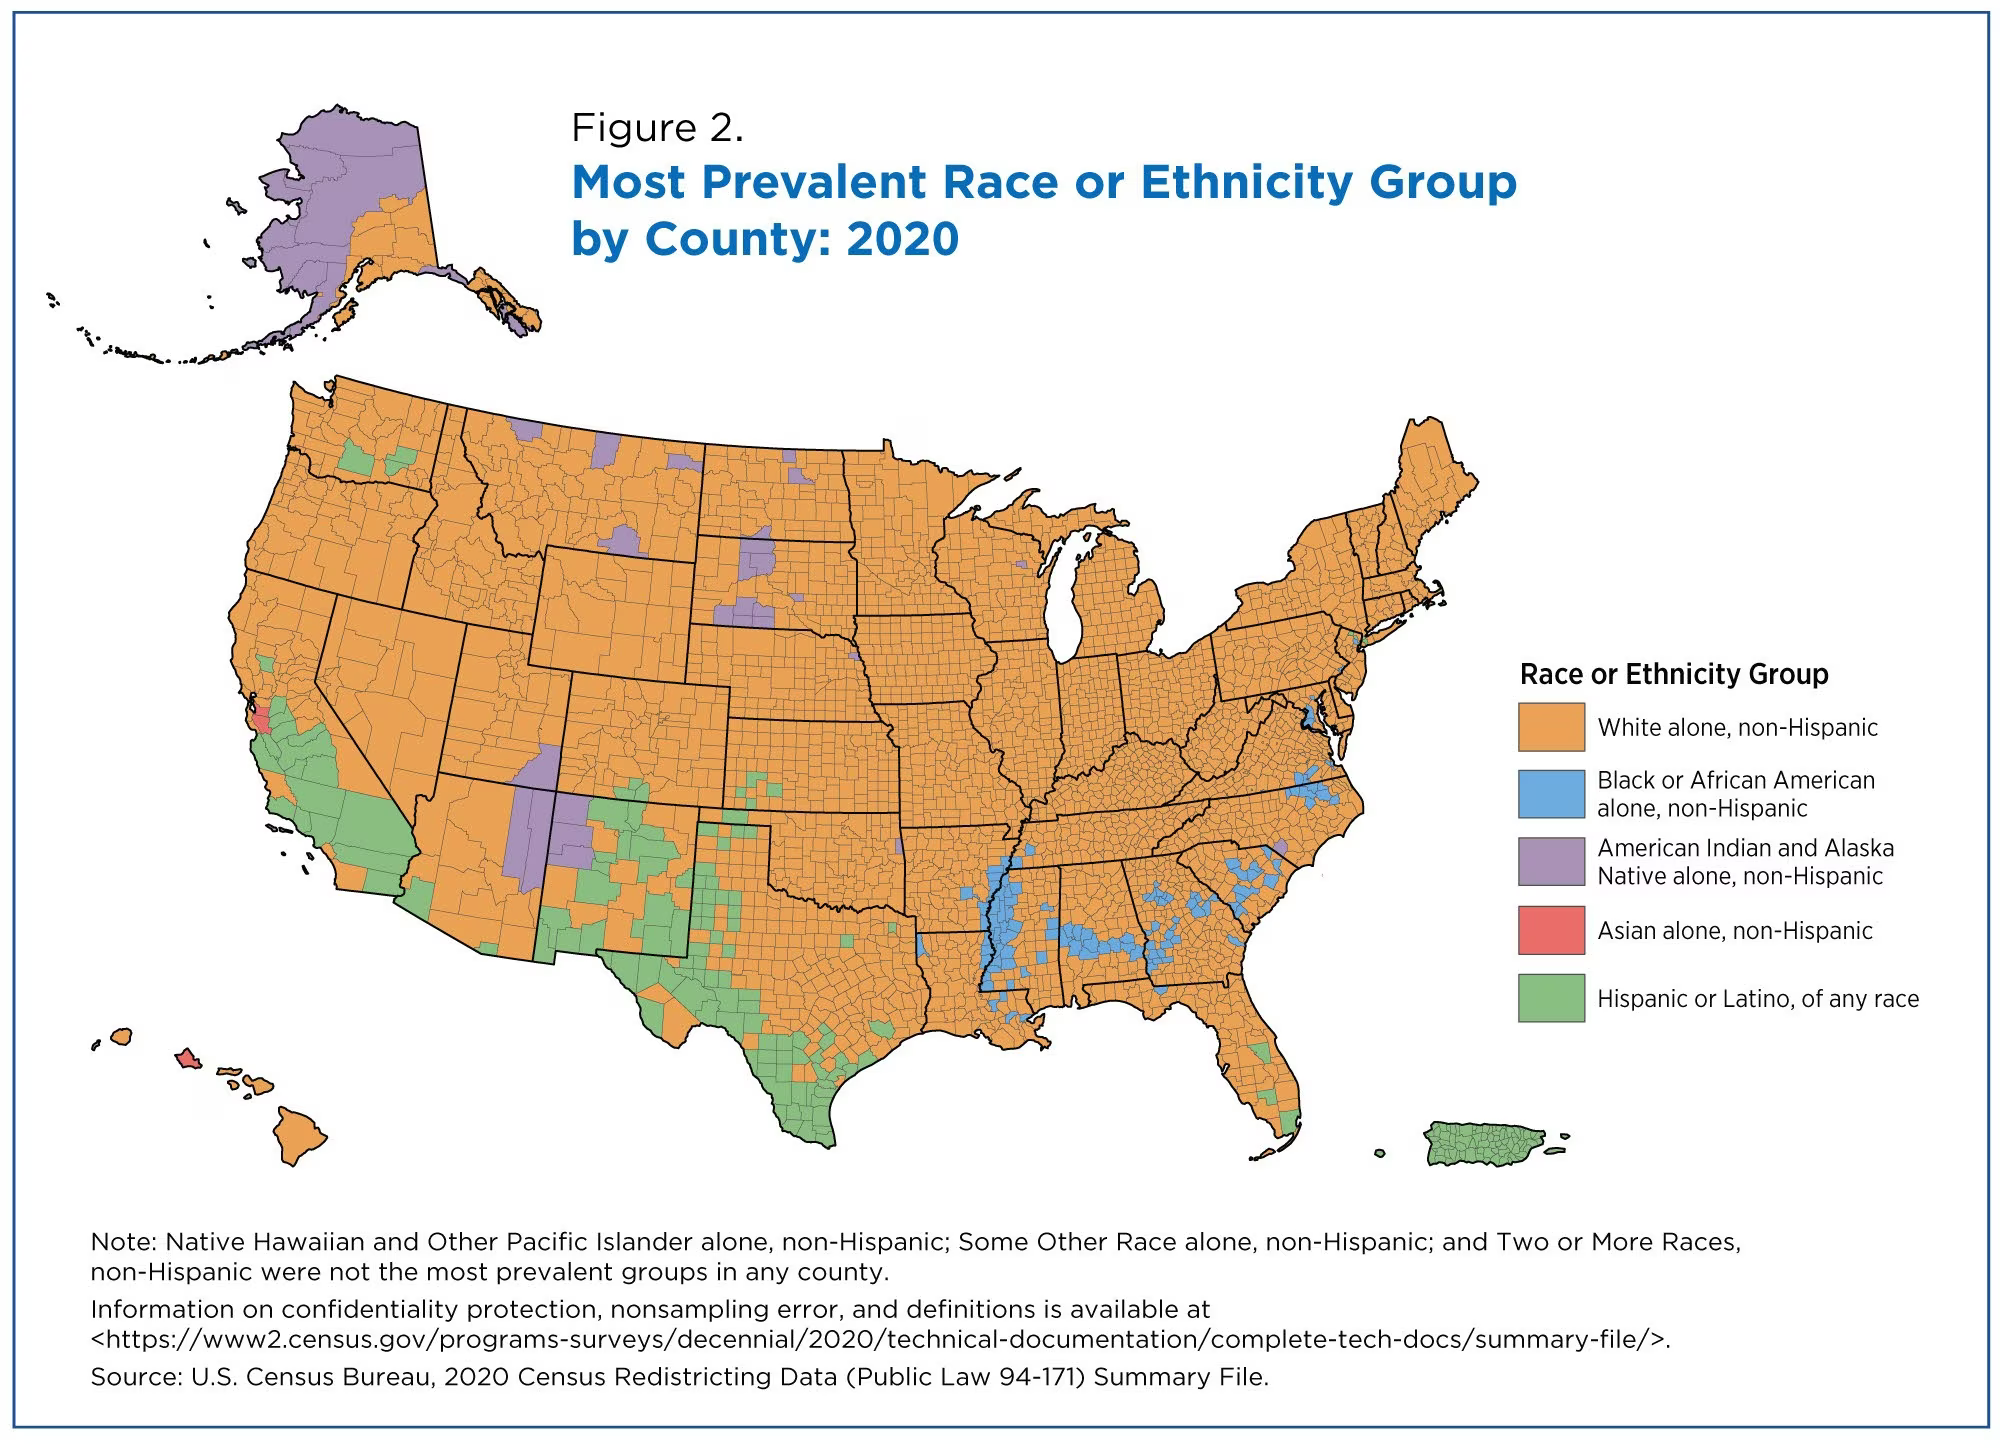
\includegraphics[width=97mm]{Imagens/2020-united-states-population-more-racially-ethnically-diverse-than-2010-figure-2.png}

    Fonte: \href{https://www.census.gov/library/stories/2021/08/2020-united-states-population-more-racially-ethnically-diverse-than-2010.html}{\textit{Bureau of the Census, 2020}}
\end{frame}

\begin{frame}
    \frametitle{OS DADOS}
    \begin{itemize}
        \item Desconsideração das taxas populacionais do país;
    \end{itemize}
    \centering
    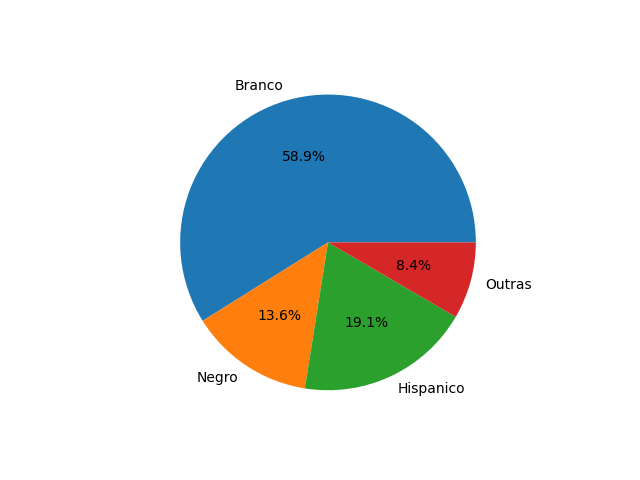
\includegraphics[width=80mm]{Imagens/Taxa Populacional Americana.png}
    
    Fonte: \href{https://www.census.gov/quickfacts/fact/table/US/}{Bureau of the Census, 2023}
    
\end{frame}

\begin{frame}
    \frametitle{OS DADOS}
    \centering
    Etnia de agressores quando a vítima é branca.
    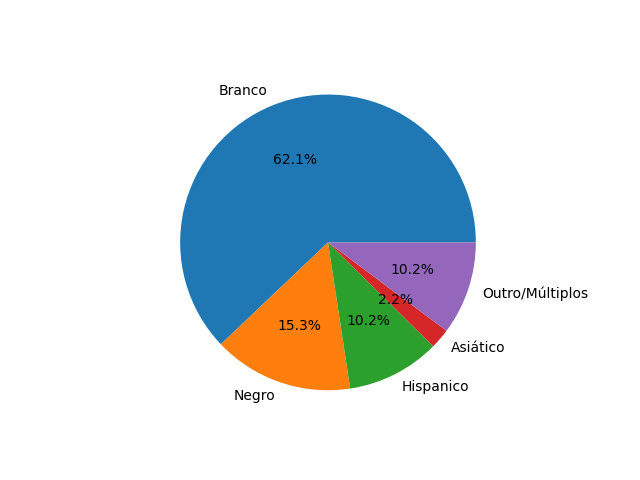
\includegraphics[width=80mm]{Imagens/Agressores Contra Brancos.png}
    
    Fonte: \href{https://bjs.ojp.gov/content/pub/pdf/cv18.pdf}{\textit{Bureau of Justice Statistics, 2018 (Criminal Victimization)}}
\end{frame}

\begin{frame}
    \frametitle{OS DADOS}
    Outros Fatores:
    \begin{itemize}
        \item A Grande maioria das comunidades brancas nos EUA não estão próximas a comunidades negras, porém, o contrário é verdadeiro (\href{https://www.nytimes.com/interactive/2015/07/08/us/census-race-map.html}{Segregação Residencial});
        \item Representação em números absolutos em detrimento a taxas;
        \item Esses crimes não são baseados na raça (\href{https://www.justice.gov/hatecrimes/learn-about-hate-crimes}{Crimes de Ódio}).
    \end{itemize}
\end{frame}

\begin{frame}
    \frametitle{CRIMES DE ÓDIO}
    \begin{columns}
    
    \column{0.5\textwidth}
        \centering
        
        \includegraphics[width=60mm]{Imagens/Crimes de Ódio 2012-2022.png}
        
    \column{0.5\textwidth}
        \centering
        
        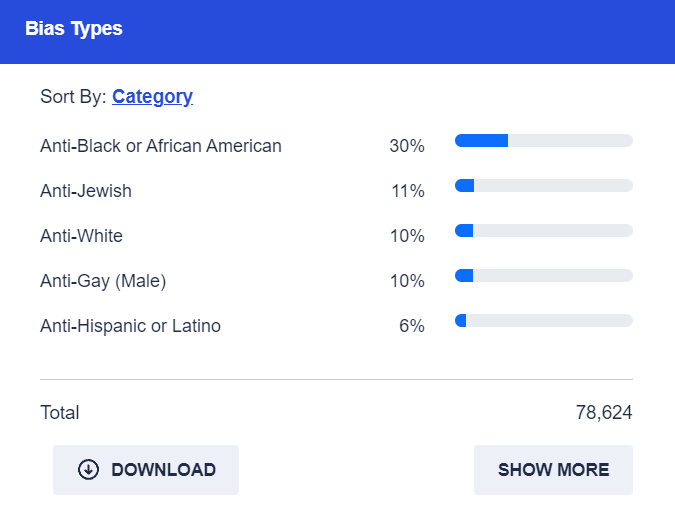
\includegraphics[width=56mm]{Imagens/Hate Crime Bias.png}
    \end{columns}

    
    \centering
    Fonte: \href{https://cde.ucr.cjis.gov/LATEST/webapp/#/pages/explorer/crime/hate-crime}{\textit{FBI, 2012-2022 (Crime Data Explorer)}}
\end{frame}

\begin{frame}[bg=Imagens/fascists.png]
\end{frame}

% FIM HENRIQUE
% INICIO DAVI
\Section{Davi}

\begin{frame}
    \frametitle{Política Tributária, Pernambuco, e Dados Reais}
    \framesubtitle{Davi Nunes}
    \textit{Plano de Governo apresentado pela atual Governadora de Perenambuco durante as eleições de 2022:}
    \begin{itemize}
        \item \textit{"Nosso Governo irá racionalizar os gastos, alavancar os investimentos para recuperar a economia e resgatar a qualidade de vida em Pernambuco."};
        \item \textit{"Iremos trabalhar para abandonar a política tributária que avançou sobre o orçamento das famílias em detrimento da renda, principalmente dos mais pobres"}.
        \newline
        \newline
    \end{itemize}
    \centering
    Fonte: \href{https://static.poder360.com.br/2022/10/Plano-de-governo-Raquel-Lyra.pdf}{Plano de Governo 2023 - 2026 (Pg. 63)}
\end{frame}

\begin{frame}
\frametitle{O Menor IPVA do Nordeste!}
\centering
\vspace{-0.5cm}
\hspace{0.5cm}
    \newline
    {\begin{tcolorbox}[newspaper]
\includegraphics[width=15mm]{Imagens/logo-jc2.webp.png} {Roberta Soares}: Como prometido, Pernambuco vai ter um dos IPVAs mais baratos do País em 2024. Nesta quarta-feira (27/12), a governadora de Pernambuco anunciou que o Imposto sobre a Propriedade de Veículos Automotores (IPVA) para o ano de 2024 será, em média, 24\% mais barato no Estado.
    A partir de janeiro, passa a valer a nova alíquota de 2,4\%, tornando Pernambuco o Estado com a menor taxação do Nordeste para esse tipo de imposto.

        \end{tcolorbox}}
   \centering
   \vspace{0.5cm}
     Fonte: \href{http://surl.li/rwukt}{Pernambuco anuncia redução média de 24\% no IPVA 2024}
\end{frame}

\begin{frame}
\frametitle{Analisando}
\begin{block}{Pontos positivos}
  \begin{itemize}
        \item \textit{Alívio Financeiro para os Proprietários de Veículos: Uma alíquota menor de IPVA significa que os proprietários de veículos precisam gastar menos dinheiro com impostos, o que pode representar uma economia significativa em seus orçamentos pessoais. }
        \item \textit{"Estímulo ao Mercado de Veículos: Alíquotas menores de IPVA podem incentivar a compra de novos veículos ou a renovação da frota, especialmente se combinadas com outras políticas governamentais favoráveis, como redução de taxas de juros para financiamentos de veículos.}.
        \newline
        \newline
    \end{itemize}
\end{block}
\end{frame}

\begin{frame}
\frametitle{Contudo}
\begin{block}{Algo está implicito}
  \begin{itemize}
        \item \textit{Por conta da Lei \href{https://l1nk.dev/i8ftt}{N° 18.305} que Modifica o artigo 15 da Lei N° 15.730 de 2016 no inciso 7 a partir de 2024 a aliquota geral que antes era de  18\% agora será de 20,5\%}
     
        \newline
        \newline
    \end{itemize}
\end{block}
\end{frame}

\begin{frame}{Pernambuco se tornou um dos Estados mais caros do Brasil!}
\centering
% Legenda da foto

% Comecei a coluna
    \begin{columns}
    
    \column{0.5\textwidth}
        \centering
        
        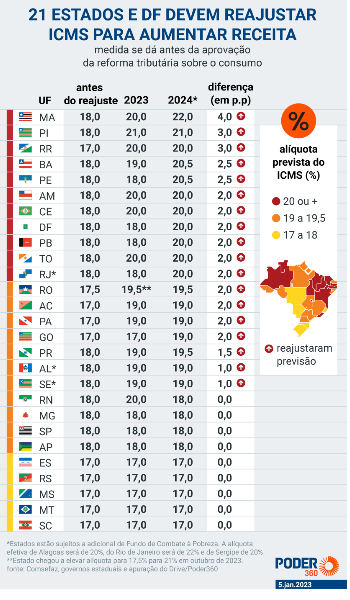
\includegraphics[width=4cm]{Imagens/Captura de tela 2024-03-24 163619.png}

        \column{0.5\textwidth}
        \centering


\begin{tcolorbox}[newspaper]
\begin{quote}
\small
\vspace{-1mm}


26 Estados e Distrito Federal começam 2024 com ICMS de 17\% a 22\%

 \\
\textit{
\includegraphics[width=4mm]{Imagens/logo-poder360-1-1.png.jpg}Hamilton Ferrari\href{https://www.poder360.com.br/economia/26-estados-e-distrito-federal-comecam-2024-com-icms-de-17-a-22/}{.}}
\end{quote}
\end{tcolorbox}
\end{columns}
\end{frame}

\begin{frame}{Pernambuco se tornou um dos Estados mais caros do Brasil!}
\centering
    \begin{columns}
    
    \column{0.5\textwidth}
        \centering
        
        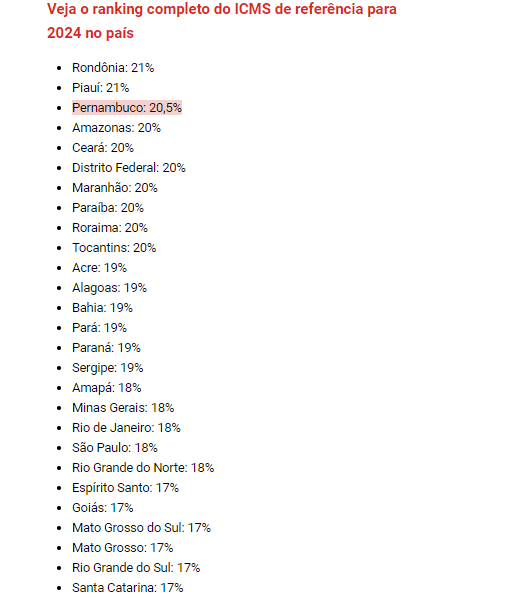
\includegraphics[width=5cm]{Imagens/Ranks de ICMS .png}
        
    \column{0.5\textwidth}
        \centering
        
        {\begin{tcolorbox}[newspaper] 
\begin{quote}
        \small
        \centering
        \vspace{0,5cm}
Aumento da atual governadora coloca Pernambuco como segundo maior ICMS do Brasil em 2024. \\
\textit{
\includegraphics[width=5mm]{Imagens/logo-jc2.webp.png} Rodrigo Fernandes\href{https://jc.ne10.uol.com.br/colunas/jamildo/2023/10/15618251-aumento-de-raquel-lyra-coloca-pernambuco-como-segundo-maior-icms-do-brasil-em-2024-veja-o-ranking.html}{.}}
        \end{quote}.

        \end{tcolorbox}}
    \end{columns}
    
\end{frame}

% FIM DAVI
% INICIO FILIPE

\Section{Filipe}

\begin{frame}
    \frametitle{Ministério da Saúde, Covid-19, e sua Letalidade}
    \framesubtitle{Luís Filipe}
    Notícia
    
    \centering
    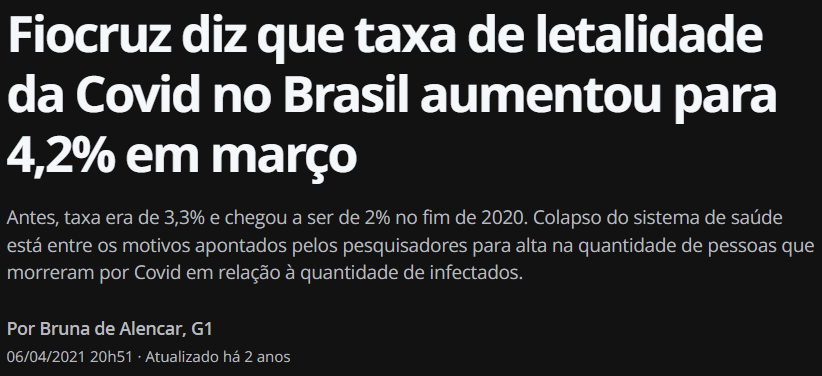
\includegraphics[width=108mm, height=50mm]{Imagens/noticiaLetalidade(2).png}

    Fonte: \href{https://g1.globo.com/bemestar/coronavirus/noticia/2021/04/06/fiocruz-diz-que-taxa-de-letalidade-por-covid-19-no-brasil-aumentou-em-marco-para-42percent.ghtml}{\textit{g1.globo}}
\end{frame}

\begin{frame}
    \frametitle{Dados}
    \textit{Dados atuais da Covid-19 no Brasil:}
    \begin{itemize}
        \item Casos confirmados: 38.694.221;
        \item Óbitos confirmados: 710.966;
        \item Letalidade: 1,8\%.
    \end{itemize}
    \centering
    Fonte: \href{https://covid.saude.gov.br}{\textit{Painel Coronavírus (Ministério da Saúde)}}
\end{frame}

\begin{frame}
    \frametitle{Problemática}
    \centering
        \begin{columns}
        
        \column{0.5\textwidth}
            \centering
            
            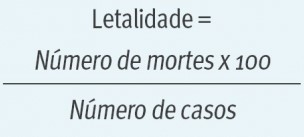
\includegraphics[width=49mm]{Imagens/letalidadeFormula.jpg}
            
        \column{0.5\textwidth}
            \centering
            
            \begin{block}{}
                \textit{Mas o número de casos pode variar em virtude:} \\
                \begin{itemize}
                    \item Das pessoas testarem mais quando já estão com sintomas;
                    \item Da eficácia do teste e do grande número de falsos positivos.
                \end{itemize}
            \end{block}
        \end{columns}
\end{frame}

\begin{frame}
    \vfill
    \begin{center}
    \centering
    \vfill
    {\fontsize{20}{25}\textit{Mas como assim eficácia?\\Ela não é considerada alta?}}
    \vfill
    \end{center}
    \vfill
\end{frame}

\begin{frame}
    \frametitle{Sim, mas...}
    \textit{Considerando o evento A = ter Covid-19 e o evento B = testar positivo, temos que:}
    \begin{itemize}
        \item O teste se preocupa com P(B|A), e quanto a isso, tem uma eficácia alta
        \item Se um teste deu positivo, queremos saber agora P(A|B), o que é completamente diferente do item anterior
    \end{itemize}
\end{frame}


% FIM FILIPE
% INICIO CARLOS

\Section{Carlos}
\begin{frame}
    \frametitle{Descontos, Golpes, Promoções, e a "Black Fraude"}
    \framesubtitle{Carlos Daniel}
    \centering
        \begin{columns}
        
        \column{0.5\textwidth}
            \centering
            
            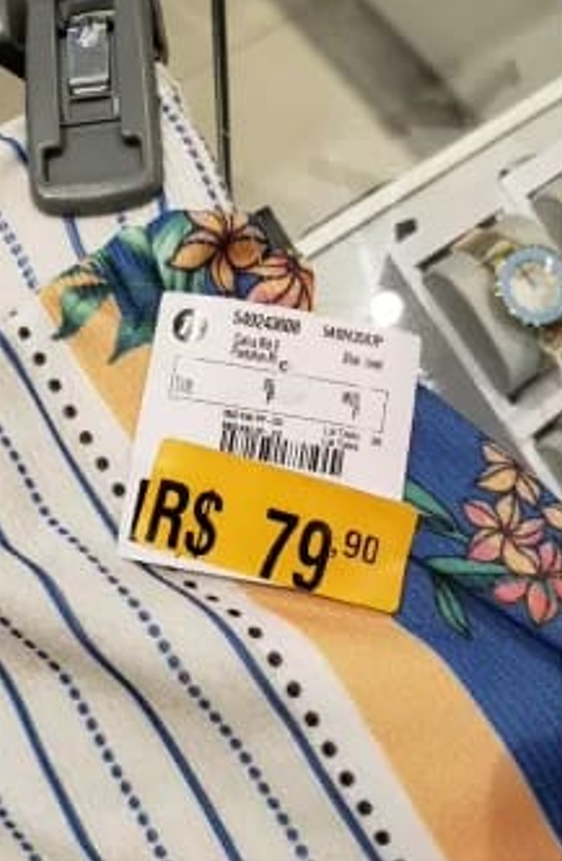
\includegraphics[width=46mm]{Imagens/blackfraude2.png}
            
        \column{0.5\textwidth}
            \centering
            
            \begin{block}{}
                \begin{itemize}
                    \item Valor Verdadeiro;
                    \item Tarja Amarela em Black Friday;
                    \item Desconto.
                \end{itemize}
            \end{block}
            Será?
            
        \end{columns}
\end{frame}

\begin{frame}
    \frametitle{"Tudo pela metade do dobro"}
    \centering
    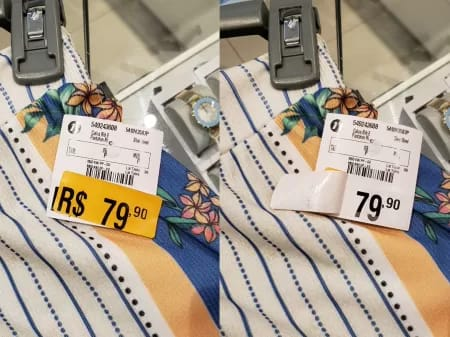
\includegraphics[width=93mm]{Imagens/blackfraude.jpg}
\end{frame}

\begin{frame}
    \frametitle{"Tudo pela metade do dobro"}
    \centering
    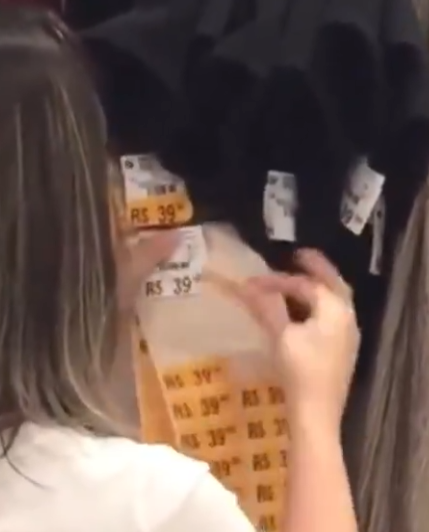
\includegraphics[width=50mm]{Imagens/adesivo.png} \\
    Fonte: \href{https://twitter.com/johnniefiveoh/status/1200008089375772672}{\textit{Postagem no X}}
\end{frame}

\begin{frame}
    \frametitle{Controvérsia}
    \framesubtitle{Renner X Procon}
    \begin{itemize}
        \item \textit{"Oi! Tudo bem? A Lojas Renner esclarece que a etiqueta amarela sinaliza os produtos participantes da Black Friday, promoção que dá desconto de 20\% nesses itens nas lojas físicas, no momento do pagamento."}
        \item \textit{"Estamos de olho. Autuamos as Lojas Renner por propaganda enganosa e precificação irregular. Vamos continuar fiscalizando, porque o seu direito é nosso dever!!"}
    \end{itemize}
    Fonte: \href{https://economia.uol.com.br/noticias/redacao/2019/11/29/empresa-se-defende-apos-video-sobre-falsa-promocao-viralizar-no-twitter.htm}{\textit{UOL Economia, 2019}}
\end{frame}

\begin{frame}
    \frametitle{Aumento Pré-Promoção}
    \framesubtitle{Dados}
    \begin{itemize}
        \item Alta nos quinze dias que antecedem a Black Friday.
        \item Monitoramento de 6.500 itens em 30 categorias;
        \item Alguns produtos ficaram até 70\% mais caros;
    \end{itemize}
    Fonte: \href{https://shorturl.at/a2456}{\textit{IBEVAR, 2020}}
\end{frame}

\begin{frame}
    \frametitle{Monitoramento dos Preços Pré-Black Friday}
    \framesubtitle{Iphone 7}
    \centering
    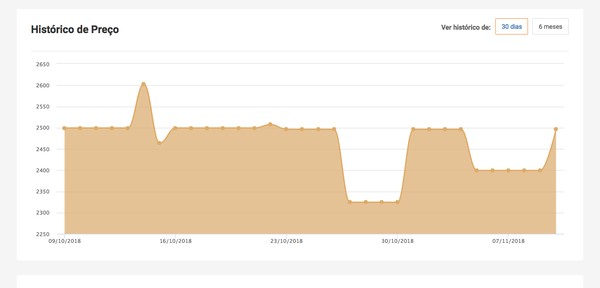
\includegraphics[width=110mm]{Imagens/iphone7.jpeg} \\
    Fonte: \href{https://www.techtudo.com.br/google/amp/noticias/2018/11/black-friday-2018-conheca-golpes-comuns-do-dia-de-descontos-e-proteja-se.ghtml}{\textit{TechTudo, 2018}}
\end{frame}
\End
\begin{frame}[plain, standout]
  \centering
  \vfill
  {\fontsize{40}{50}\selectfont OBRIGADO}
  \vfill
  \begin{center}
    
\includegraphics[scale=0.03]{Imagens/FGV-Logo.png}
  \end{center}
\end{frame}

\end{document}
